% !TeX spellcheck = de_DE
\documentclass[ngerman,12pt]{article}

% Packages for Language
\usepackage[ngerman]{babel}
\usepackage[utf8]{inputenc}
\usepackage[T1]{fontenc}
\usepackage[final]{graphicx}
\usepackage{amsmath}
\usepackage{float}
%\usepackage{wrapfig}
\usepackage{caption}
%\usepackage{multirow}
\usepackage{subfig}
\usepackage{hyperref}
\usepackage[german, plain]{fancyref}
\usepackage{afterpage,pdflscape} %%% !!!!!!! CHANGE TO PDFLSCAPE LATER!
\usepackage{varioref}
\usepackage{siunitx}
\usepackage{translator}
\usepackage{listings}
\usepackage{fancyhdr}
\pagestyle{fancy}
\usepackage[de-DE]{datetime2}
\DTMsetdatestyle{dmyyyy}

%\usepackage{showframe}

\setlength{\headheight}{15.5pt}
\lhead{NAME NAME NAME}
\rhead{\today}
\chead{Numerik Übung 10}


\begin{document}
\lstset{language=Matlab,basicstyle=\ttfamily,columns=fixed}
\subsubsection*{midpoint.m}
\begin{lstlisting}[frame=single]
function [ I ] = midpoint( f,a,b,N )
h=(b-a)/N;
x=a:h:b;
x=x(1:end-1)+h/2;
fx=f(x);
I=h*sum(fx);
end
\end{lstlisting}

\subsubsection*{trapez.m}
\begin{lstlisting}[frame=single]
function [ I ] = trapez( f,a,b,N )
h=(b-a)/N;
x=a:h:b;
fx=f(x);
I=(h/2)*(fx(1)+fx(end))+h*sum(fx(2:end-1));
end
\end{lstlisting}

\subsubsection*{main.m}
\begin{lstlisting}[frame=single]
f = @(x) sqrt(4.*cos(x).^2+sin(x).^2);

approx = 9.688448220547674;

for N=1:30;
  midpointR(N) = midpoint(f,0,2*pi,N);
  trapezR(N) = trapez(f,0,2*pi,N);
end

semilogy(1:30,abs(approx-rm),1:30,abs(approx-rt));
legend('Midpoint', 'Trapez');
\end{lstlisting}
%\filbreak


\subsubsection*{Fehlerplot}
\begin{figure}[H]
    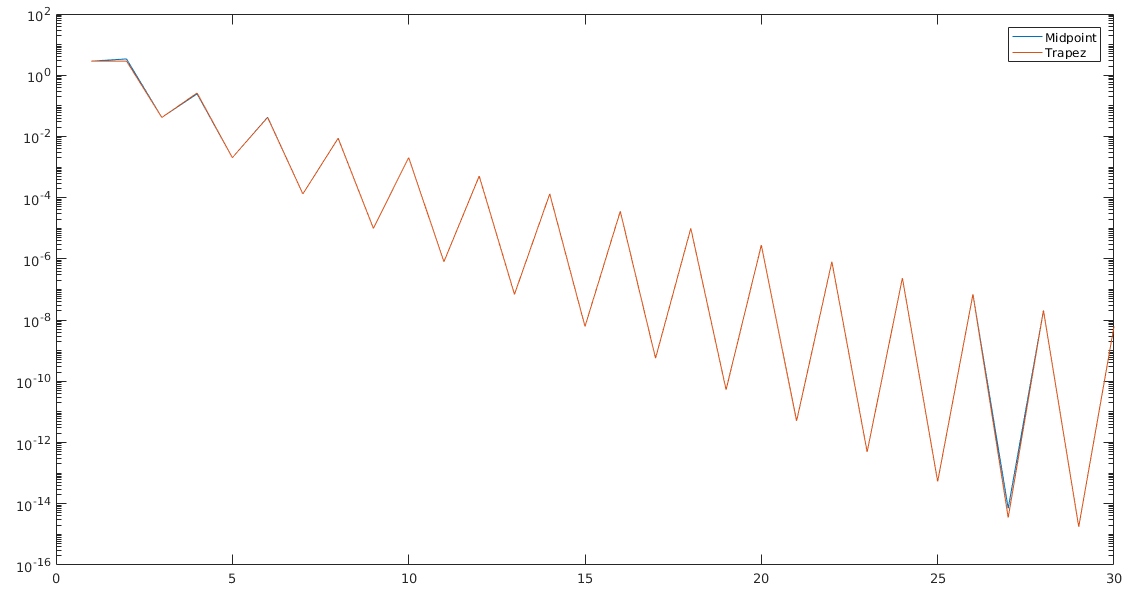
\includegraphics[width=\linewidth,keepaspectratio]{result_crop.png}
\end{figure}



\end{document}